\documentclass{exam}

\usepackage{indentfirst}
\usepackage{url}
\usepackage{graphicx}
\usepackage{listings}
\usepackage{color}
\usepackage{fancyvrb}

\definecolor{mygreen}{rgb}{0,0.6,0}
\definecolor{mygray}{rgb}{0.5,0.5,0.5}
\definecolor{mymauve}{rgb}{0.58,0,0.82}

\lstset{ %
  backgroundcolor=\color{white},		% choose the background color; you must add \usepackage{color} or \usepackage{xcolor}
  basicstyle=\small\ttfamily,		% the size of the fonts that are used for the code
  breakatwhitespace=false,			% sets if automatic breaks should only happen at whitespace
  breaklines=true,					% sets automatic line breaking
  captionpos=b,						% sets the caption-position to bottom
	columns=fullflexible,
  commentstyle=\color{mygreen},		% comment style
  deletekeywords={...},				% if you want to delete keywords from the given language
  escapeinside={\%*}{*)},			% if you want to add LaTeX within your code
  extendedchars=true,				% lets you use non-ASCII characters; for 8-bits encodings only, does not work with UTF-8
  frame=single,						% adds a frame around the code
  keepspaces=true,					% keeps spaces in text, useful for keeping indentation of code (possibly needs columns=flexible)
  keywordstyle=\color{blue},			% keyword style
  language=Octave,					% the language of the code
  morekeywords={*,...},				% if you want to add more keywords to the set
%   numbers=left,						% where to put the line-numbers; possible values are (none, left, right)
%   numbersep=6pt,						% how far the line-numbers are from the code
%   numberstyle=\tiny\color{mygray},	% the style that is used for the line-numbers
  rulecolor=\color{black},			% if not set, the frame-color may be changed on line-breaks within not-black text (e.g. comments (green here))
  showspaces=false,					% show spaces everywhere adding particular underscores; it overrides 'showstringspaces'
  showstringspaces=false,			% underline spaces within strings only
  showtabs=false,					% show tabs within strings adding particular underscores
  stepnumber=1,						% the step between two line-numbers. If it's 1, each line will be numbered
  stringstyle=\color{mymauve},		% string literal style
  tabsize=2,							% sets default tabsize to 2 spaces
  title=\lstname						% show the filename of files included with \lstinputlisting; also try caption instead of title
}

% Creates a new command to include a perl script, the first parameter is the filename of the script (without .pl), the second parameter is the caption
\newcommand{\octavescript}[2]{
\lstinputlisting[caption=#2,label=#1]{#1}
}

\newcommand{\MNLab}{Laborator\ \#1}
\newcommand{\MNLabTitle}{Introducere în MATLAB. Funcții și instrucțiuni. Vizualizarea datelor.} 
\newcommand{\MNAuthor}{Andrei STAN, Bogdan Țigănoaia}

\renewcommand{\contentsname}{Cuprins}
\renewcommand{\figurename}{Figura}

\setlength{\parskip}{0.5\baselineskip}

\graphicspath{{./img/}}

\title{
\textmd{\textbf{\MNLabTitle}}
\author{Colaboratori: \MNAuthor}
}

\pagestyle{headandfoot}

\header{Metode Numerice}
{Introducere in MATLAB, Pagina \thepage\ din \numpages}
{2025}
\footer{Facultatea de Automatică și Calculatoare}{}{Pagina \thepage\ din \numpages}

\begin{document}

\begin{coverpages}

	\maketitle
	\tableofcontents

\end{coverpages}

\section{Obiective laborator}

În urma parcurgerii acestui laborator, studentul va fi capabil să:
\begin{itemize}
	\item utilizeze MATLAB/Octave pentru a rezolva probleme de calcul numeric;
	\item folosească fișiere \verb|.m|;
	\item folosească funcții predefinite, funcții de citire/scriere de tipul C.
\end{itemize}

\section{Noțiuni teoretice}

\subsection{Ce este MATLAB?}

\par Modelarea problemelor matematice în sistemele informatice se poate face cu
ajutorul \textit{programelor specializate pentru calcule matematice}
(Mathematica\footnote{\url{https://www.wolfram.com/mathematica/}},
MathCAD\footnote{\url{https://www.ptc.com/product/mathcad}}) sau cu ajutorul
\textit{mediilor de programare} (MATLAB\footnote{\url{https://www.mathworks.com/products/matlab/}},
Maple\footnote{\url{https://www.maplesoft.com/products/maple/}},
Octave\footnote{\url{https://www.gnu.org/software/octave/}},
Scilab\footnote{\url{https://www.scilab.org}}).
Vă recomandăm și portalul WolframAlpha\footnote{\url{https://www.wolframalpha.com}}.

\par MATLAB (MATrix LABoratory) este un limbaj de programare, cât și o suită
software, special construit pentru calcul numeric, vizualizare de date,
procesarea semnalelor, etc.
Utilitatea limbajului constă că este bazat pe folosirea matricilor: toate datele sunt reprezentate sub forma unor matrici. Asta înseamnă că putem lucra mult mai ușor cu numerele, dar și mai rapid, toate operațiile fiind optimizate.
Pentru vizualizare ne sunt puse la dispoziție numeroase funcții pentru crearea graficelor atât 2D, cât și 3D.

\subsection{Software necesar}

\par Recomandăm folosirea GNU Octave pentru parcurgera laboratoarelor, cât și a temelor.

\par Mult mai puternică este suita de la MathWorks: \url{https://matlab.mathworks.com/}.
Pentru autentificare, folosiți mail-ul instituțional.
Universitatea oferă deja licență tuturor. Mediul online este suficient pentru
acest curs.

\newpage
\subsection{Interfața Octave}

\begin{figure}[ht]
	\centering
	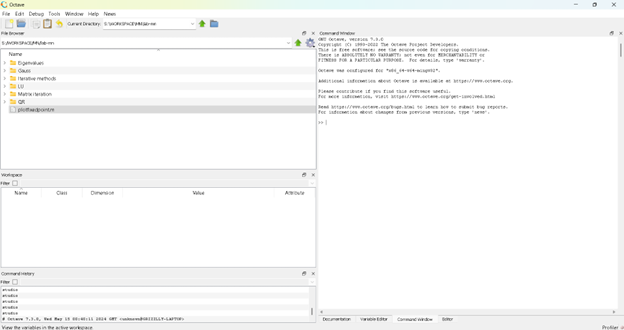
\includegraphics[width=0.9\textwidth]{interf}
	\caption{Interfața Octave}
\end{figure}

\par Limbajul este similar cu Python, fiind unul interpretat. În partea de sus
vedem directorul curent (cel în care se vor rula comenzile).

\par În partea stângă avem 3 panouri:

\begin{itemize}
	\item \textbf{File Browser} - unde putem naviga prin fișiere;
	\item \textbf{Workspace} - unde sunt stocate variabilele;
	\item \textbf{Command History} - istoricul comenzilor.
\end{itemize}

\par În partea dreaptă avem 4 panouri:

\begin{itemize}
	\item \textbf{Cocumentation} - unde putem căuta ajutor;
	\item \textbf{Variable Editor} - unde putem modifica variabilele;
	\item \textbf{Command Window} - unde putem rula comenzile;
	\item \textbf{Editor} - unde putem scrie codul.
\end{itemize}

\subsection{Introducere în MATLAB}

\par De acum, pentru rularea comenzilor vom folosi \textit{Command Window}.

\subsubsection{Comenzi}

\par Toate comenzile se execută în dircetorul curent. Putem folosi comanda \verb|pwd|
pentru a vedea directorul curent.

\newpage
\par Rezultatul unui calcul se va stoca mereu în variabila \verb|ans|:

\begin{figure}[ht]
	\centering
	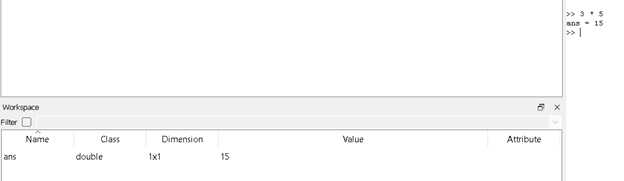
\includegraphics[width=0.9\textwidth]{ans}
	\caption{Variabila ans}
\end{figure}

\par Variabilele se crează prin atribuire:

\begin{lstlisting}
>> m = 3 * 5
>> y = m / 2
\end{lstlisting}

\par După rularea comenzilor, obervați că mereu se afișează rezultatul. Pentru a
nu afișa rezultatul, folosiți \verb|;| la sfârșitul comenzii.

\begin{lstlisting}
>> m = 3 * 5;
>> y = m / 2;
\end{lstlisting}

\subsubsection{Manipularea matricelor}

\par MATLAB este un limbaj orientat pe matrici. Toate operațiile sunt făcute pe
matrici. Scalarii sunt considerați matrici de dimensiune 1x1. Pentru a crea o
matrice sau un vector putem folosi construcțiile de mai jos:

\begin{lstlisting}
>> A = [1 2 3; 4 5 6; 7 8 9] % matrice 3x3
>> B = [1 2 3] % vector linie
>> C = [1; 2; 3] % vector coloana
\end{lstlisting}

\par Pentru crearea vectorilor cu elemente egal depărtate, putem folosi
construcția \verb|start : step : end|:

\begin{lstlisting}
>> D = 1 : 2 : 10 % vector cu elemente de la 1 la 10, cu pasul 2
>> E = 1 : 5 % vector cu elemente de la 1 la 5, pasul a fost omis (implicit 1)
\end{lstlisting}

\par Operatorii care acționează pe matrici sunt:

\begin{itemize}
	\item \verb|+| - adunare;
	\item \verb|-| - scădere;
	\item \verb|*| - înmulțire;
	\item \verb|/| - împărțire;
	\item \verb|'| - transpusa (hermitica);
	\item \verb|.| - operatorul Hadamard (execută operația element cu element).
\end{itemize}

\par Prin împărțirea unei matrici la alta, se înțelege înmulțirea primei cu
inversa celei de-a doua. De exemplu, pentru rezolvarea sistemului $Ax = b$, se
poate folosi formula $x = A \backslash b$.

\par Exemplul de mai jos folosește operatorul Hadamard, rezultatul fiind
matricea \verb|A = [1 4; 9 16]|:

\begin{lstlisting}
>> A = [1 2; 3 4];
>> B = A .^ 2
\end{lstlisting}

\par Pentru a afla dimensiunile unei matrici, folosim funcția \verb|size|. Aceasta
va returna un vector cu mai multe elemente, fiecare reprezentând lungimea unei
dimensiuni.

\par Accesarea elementelor unei matrici se face folosind indicii (începând de la 1):

\begin{lstlisting}
>> A = [1 2 3; 4 5 6; 7 8 9];
>> A(2, 3) % elementul de pe linia 2, coloana 3
>> A(2, :) % linia 2
>> A(:, 2) % coloana 2
>> A(1 : 2, 1 : 2) % submatricea formata din primele 2 linii si primele 2 coloane
>> A([1 3], :) % liniile 1 si 3
\end{lstlisting}

\subsubsection{Salvarea și încărcarea datelor}

\par Pentru a salva spațiul de lucru curent, adică toate variabilele și
valorile lor, putem folosi comanda \verb|save|:

\begin{lstlisting}
>> save nume_fisier.mat
\end{lstlisting}

\par Pentru a încărca datele salvate, folosim comanda \verb|load|:

\begin{lstlisting}
>> load nume_fisier.mat
\end{lstlisting}

\par Pentru a șterge o variabilă din spațiul de lucru, folosim comanda
\verb|clear|:

\begin{lstlisting}
>> clear nume_variabila
\end{lstlisting}

\subsubsection{Funcții și variabile predefinite}

\par MATLAB vine cu o mulțime de funcții și variabile predefinite. De exemplu,
constanta \verb|pi|, funcțiile \verb|sin|, \verb|cos|, \verb|tan|, \verb|exp|,
\verb|log|, \verb|sqrt|, \verb|abs|, \verb|round|, \verb|floor|, \verb|ceil|.

\begin{lstlisting}
>> pi / 2
% output: 1.5708
\end{lstlisting}

\par Chiar dacă sunt afișate doar 4 zecimale, MATLAB folosește o precizie de
16 zecimale.

\par O particularitate foarte frumoasă a funcțiilor este că acestea pot fi
aplicate pe vectori, rezultatul fiind un vector cu aceeași dimensiune. Mai
târziu vom prezenta conceptul de \textit{vectorizare} și de ce e bine să scriem
cod așa și nu cu bucle.

\begin{lstlisting}
>> A = [0 pi/2 pi 3*pi/2 2*pi];
>> sin(A)
% output: [0 1 0 -1 0]
\end{lstlisting}

\subsubsection{Script-uri}

\par Un script este un fișier care conține o secvență de comenzi MATLAB. Acesta
are extensia \verb|.m|. Pentru a rula un script, putem folosi GUI-ul Octave
apăsând pe butonul \textit{Run} sau putem folosi linia de comandă scriind numele
fișierului fără extensie.

\par Într-un script putem folosi toate comenzile pe care le-am folosit în
\textit{Command Window}. De exemplu, scriptul de mai jos va afișa pe ecran
numerele de la 1 la 10:

\begin{lstlisting}
for i = 1 : 10
	disp(i);
endfor % sau end
\end{lstlisting}

\subsubsection{Instrucțiuni de control}

\par MATLAB suportă instrucțiuni de control precum \verb|if|, \verb|for|,
\verb|while|, \verb|switch|. Sintaxa este similară cu cea din alte limbaje de
programare.

\begin{lstlisting}
if conditie
	% cod
elseif conditie
	% cod
else
	% cod
endif % sau end
\end{lstlisting}

\begin{lstlisting}
for i = 1 : 10 % for poate opera pe orice vector, variabila i va lua valorile pe rand
	% cod
endfor % sau end
\end{lstlisting}

\begin{lstlisting}
while conditie
	% cod
endwhile % sau end
\end{lstlisting}

\begin{lstlisting}
switch variabila
	case valoare1
		% cod
	case valoare2
		% cod
	otherwise
		% cod
endswitch % sau end
\end{lstlisting}

\subsubsection{Funcții definite de utilizator}

\par Funcțiile sunt secvențe de comenzi care primesc unul sau mai mulți
parametri și întorc un rezultat. Pentru modularizrea codului, este bine să
scriem fiecare funcție într-un fișier separat. Acest fișier va avea aceeași
denumire cu funcția, dar cu extensia \verb|.m|.

\par Creați fișierul \verb|suma.m| cu următorul conținut:

\begin{lstlisting}
function s = suma(a, b)
	s = a + b;
endfunction
\end{lstlisting}

\par Testați apelurile funcției \verb|suma(1, 2)| și \verb|suma(1 : 2, 3 : 4)|.

\par Putem avea și funcții void (care nu întorc nimic) folosind
\verb|function [] = nume_functie()| sau funcții care întorc mai multe valori
folosind \verb|[a, b, c, d] = nume_functie()|.

\subsubsection{Vectorizări}

\par MATLAB este optimizat pentru operațiile pe matrici. De aceea, este bine să
folosim cât mai puține bucle în codul nostru. Acest lucru se numește
\textit{vectorizare}. De exemplu, în loc să scriem:

\begin{lstlisting}
for i = 1 : 10
	y(i) = x(i) ^ 2;
endfor
\end{lstlisting}

\par Putem scrie:

\begin{lstlisting}
y = x .^ 2;
\end{lstlisting}

\par În continuare, vom prezenta câteva exemple de vectorizare dar și de alte
funcții și construcții utile.

\newpage
\par Exemplul 1:

\begin{lstlisting}
x = -2 : 0.5 : 2;
for i = 1 : length(x)
	if x(i) >= 0
		s(i) = sqrt(x(i));
	else
		s(i) = 0;
 	endif
endfor
\end{lstlisting}

\begin{lstlisting}
x = -2 : 0.5 : 2;
s = sqrt(x);
s(x < 0) = 0
\end{lstlisting}

\par În acest exemplu, ne-am bazat pe faptul că funcția \verb|sqrt| primește ca
parametrii și numere negative, având ca rezultat un numar complex. Am folosit
operatorul \verb|<| care aplicat vectorilor are ca rezultat un alt vector cu 1
pe pozițiile ce satisfac condiția. Mai mult, am utilizat indexarea unui vector
prin intermediul altui vector.

\par Exemplul 2:

\begin{lstlisting}
M = magic(3);
for i = 1 : 3
	for j = 1 : 3
		if (M(i, j) > 4),
			M(i, j) = -M(i, j);
		endif
	endfor
endfor
\end{lstlisting}

\begin{lstlisting}
M = magic(3);
ind = find(M > 4); % returneaza indicii elementelor care satisfac conditia
M(ind) = -M(ind)
\end{lstlisting}

\par În acest exemplu, secvența care folosește bucla for se execută în 23.4956
unități de timp iar secvența vectorizată, prin intermediul funcției find, se
execută în 2.1153 unități de timp, deci de 11 ori mai rapid.

\par Exemplul 3:

\begin{lstlisting}
for i = 1 : n
	for j = 1 : n
		M(i, j) = A(i, j) / (B(i, j) * C(i, j));
	endfor
endfor
\end{lstlisting}

\begin{lstlisting}
M = A ./ (B .* C)
\end{lstlisting}

\par În acest exemplu, am folosit operatorul Hadamard pentru eliminarea buclelor.

\subsubsection{Vizualizarea datelor}

\par MATLAB vine cu o mulțime de funcții pentru vizualizarea datelor. În
laboratoarele următoare vom folosi aceste funcții pentru a vizualiza rezultatele
obținute.

\par Funcția \verb|plot| este folosită pentru a crea grafice 2D. Aceasta
primește ca parametrii doi vectori, unul pentru axa x și unul pentru axa y. De
asemenea, putem adăuga și alți parametrii pentru a personaliza graficul. Pentru
mai multe detalii privind parametrii, consultați documentația.

\octavescript{./src/plot1.m}{}

\begin{figure}[ht]
	\centering
	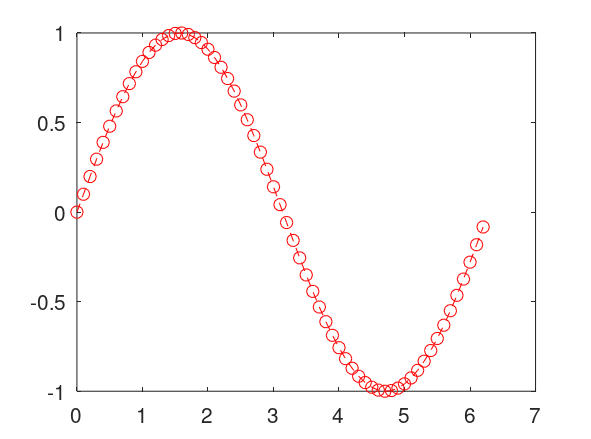
\includegraphics[width=0.9\textwidth]{plot1}
	\caption{Funcția $sin(x)$ evaluată pe intervalul $[0, 2 * \pi]$, cu pas $0.1$.}
\end{figure}

\newpage
\par Pentru a trasa graficele funcțiilor multiple, putem folosi aceeași funcție
\verb|plot|, dar cu mai mulți parametrii.

\octavescript{./src/plot2.m}{}

\begin{figure}[ht]
	\centering
	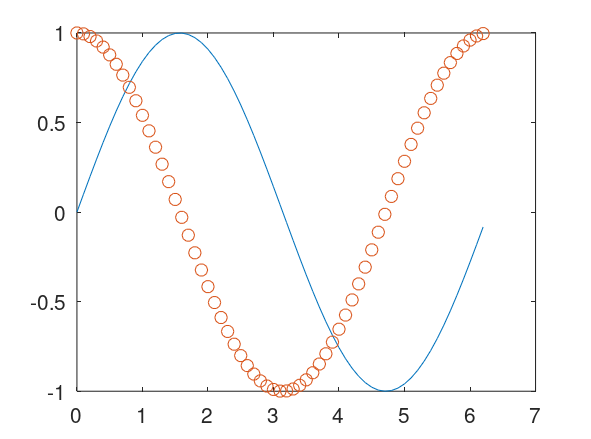
\includegraphics[width=0.9\textwidth]{plot2}
	\caption{Funcția $sin(x)$ trasată prin interpolare liniară și funcția $cos(x)$ trasată prin puncte.}
\end{figure}

\section{Probleme}

\begin{questions}
	\boxedpoints
	\pointsinmargin

	\question Creați câte un script pentru funcțiile $f(x) = x^2$, $g(x) = x^3$
	și $h(x) = x^4$.
	Trasați graficele acestora pe intervalul $[-10, 10]$.

	\question Construiți vectorul $x$ cu elemente de la $0$ la $10$ cu pasul $3$.
	Construiți vectorul $y = sin(i), i \in x$. Trasați graficul rezultat din cei
	doi vectori. Rulați script-ul cu pași din ce în ce mai mici pentru $x$. Ce
	observați?
\end{questions}

\end{document}
